\chapter{脾}

\section{检查方法}

\subsection{扫描前准备}

一般扫描前口服2%的泛影葡胺500~800ml,使胃肠道充盈。

\subsection{扫描方法}

1.平扫:自膈肌开始,以5~10mm层厚与间距行连续扫描。螺旋CT可采用3~10mm的准直,螺距1~2∶1。

2.增强扫描:静脉团注60%造影剂100ml,作快速或动态扫描,脾明显强化。因此,可以鉴别病灶是原发于脾或附近脏器如胃、胰、肾上腺或肾。但部分患者在静脉早期由于脾脏呈不均匀强化,可遗漏小的病变,稍后脾脏强化密度即逐渐趋向一致。

近年来推出的脂融性造影剂如EOE-13选择性的只被肝、脾网状内皮细胞所吸收,特异性强、增强效果好。但毒性强,尚较少应用。

\section{正常解剖、先天变异和畸形}

\subsection{大小和密度}

1.形态:脾位于左膈下,其位置也可因个人情况而不同,如脾周围韧带松弛可位置较低。外缘圆隆而光滑,伴9~11肋骨下行。内缘因胃、胰及肾造成的压迹而呈分叶状隆起,不同层面有不同的外形。正常脾内缘可见1至数个小切迹,脾下缘亦可有切迹。脾门部可见大血管出入。

在较深切迹的扫描层面,脾脏可形似完全离断,但上下层面仍可见切迹两侧的脾是相连的。

最常见的隆起夹在胰尾和左肾上极之间,可形似肾上腺、肾或胰尾部肿块,尤其脾大时多见。

2.大小:脾的大小因不同年龄、体重及营养状况而不同。一般成人脾脏长12cm,宽7cm,厚约3~4cm。长>15cm肯定增大,脾厚>4.5cm可视为增大。此外,脾脏的下缘超过正常肝脏的下缘或脾脏前后径超过腹部前后径的2/3均提示脾大。

3.密度:正常脾脏密度均匀,其CT值正常范围较大,平扫时总低于正常肝脏约5~10Hu。增强扫描早期皮质强化高于中间髓质而致密度不均,稍后密度均匀,CT值可达100~150Hu。

\subsection{副脾}

副脾是一种并不少见的先天性变异,由正常脾组织构成,尸检时发现副脾占10%~30%,与创伤所引起的异位脾组织种植不同。

\textbf{【病理】}
副脾呈球形,最常见于脾门附近;少数靠近胰尾;罕见于其他部位如胃壁、小肠壁、大网膜、肠系膜、横膈甚至盆腔内或阴囊内。可与脾完整分离,亦可与主脾有一细蒂相连。单个或多个,通常不超过6个。副脾多由脾动脉供血,有脾门和正常结构的包膜。

\textbf{【CT表现】}
①呈单发或多发的、边缘光滑的圆形或卵圆形结节影(图\ref{fig14-1}、图\ref{fig14-2});②密度均匀且与脾实质密度相同;③动态增强扫描与脾同时增强和消退,CT值与脾相同;④不典型部位者需结合超声等观察其血供来源等综合诊断。

\begin{figure}[!htbp]
 \centering
 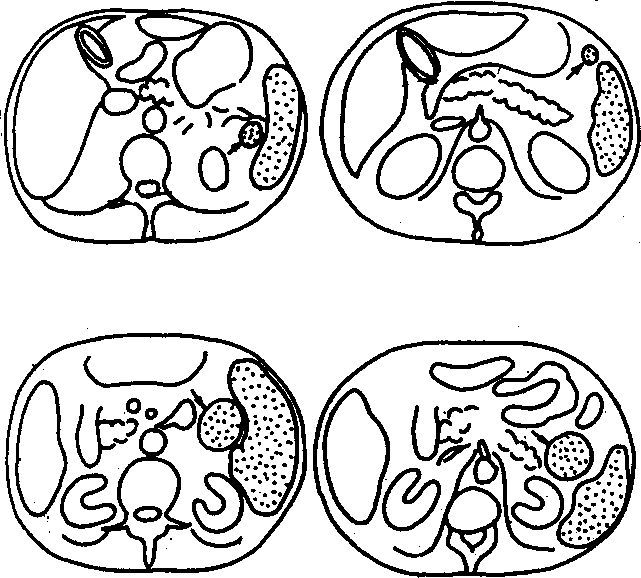
\includegraphics[width=.7\textwidth,height=\textheight,keepaspectratio]{./images/Image00309.jpg}
 \captionsetup{justification=centering}
 \caption{副脾的各种表现}
 \label{fig14-1}
  \end{figure} 

\begin{figure}[!htbp]
 \centering
 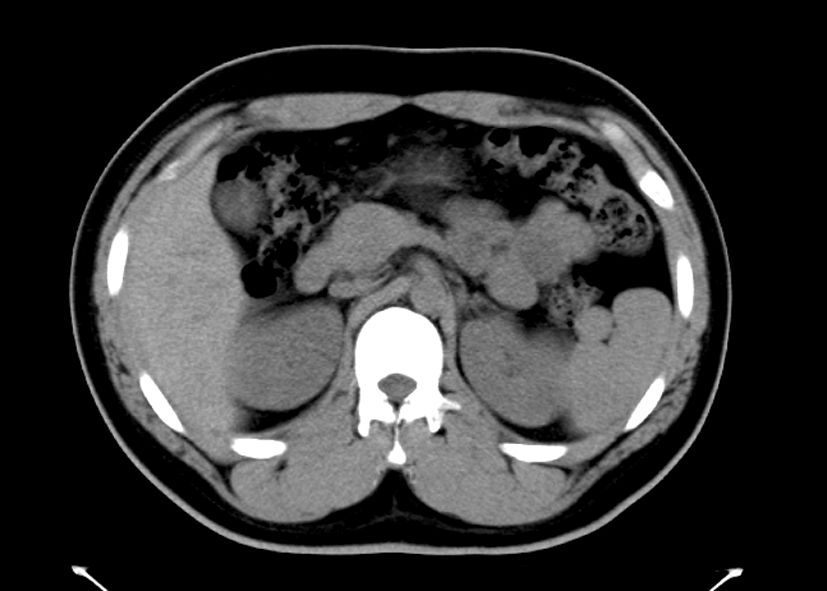
\includegraphics[width=.7\textwidth,height=\textheight,keepaspectratio]{./images/Image00310.jpg}
 \captionsetup{justification=centering}
 \caption{副 脾\\{\small 左侧脾门下方有圆形软组织密度结节,与脾密度一致,边缘光滑}}
 \label{fig14-2}
  \end{figure} 

识别副脾的意义:①脾亢等病在脾切除后,副脾可以明显增大并引起原发症状的复发,因此应把副脾一并切除;②勿将副脾误为增大淋巴结或肿瘤;③脾脏肿瘤亦可累及到副脾,如淋巴瘤;④副脾少见的并发症是自发性破裂、梗死或扭转。

\subsection{游走脾}

本病亦称为异位脾、迷走脾、脾下垂或漂浮脾。

\textbf{【病因】}
尚有争论,大多认为是一种少见的先天性异常,由于支持脾脏的韧带松弛或缺如所致。但亦有学者认为还存在着继发因素,包括脾大、创伤及妊娠时内分泌作用和腹部松弛等。

\textbf{【临床表现】}
可发生于6~80岁,以20~40岁的女性多见。病人可无症状而偶然发现。由于急性或慢性扭转可引起急腹症、脾梗死、脾坏疽、脓肿、胃食管静脉曲张、脾淤血、脾大、脾功能亢进等。

\textbf{【CT表现】}
可显示在胃后方和左肾前方的脾缺如。在下腹部或盆腔内可见一个密度均匀的实质性“肿块”,相当于脾脏大小;增强扫描符合正常脾组织的强化规律。如有扭转存在,可有脾梗死表现;如扭转累及胰尾,可导致胰尾坏死和腹水;如慢性扭转病例,可见增厚和强化的假包膜,由网膜和腹膜粘连形成。

\subsection{无脾和多脾综合征}

无脾和多脾可为孤立性表现,但常常伴先天性心血管异常和内脏位置异位,分别称为无脾综合征和多脾综合征。

\textbf{【CT表现】} 常见表现如下:

1.无脾综合征:①肺部畸形:双侧呈三叶肺(右肺形态)、双侧右支气管型表现等;②腹部内脏位置异常和畸形,以及脾缺如;③增强扫描见主动脉和下腔静脉位于同一侧可提示无脾综合征,而本征很少见到下腔静脉肝段缺如伴奇静脉连接。

2.多脾综合征:①肺部畸形:双侧呈二叶肺(左肺形态);②腹部内脏位置异常和畸形;③右侧多个小脾、下腔静脉肝段缺如伴奇静脉连接等为其特征性征象(图\ref{fig14-3})。

\begin{figure}[!htbp]
 \centering
 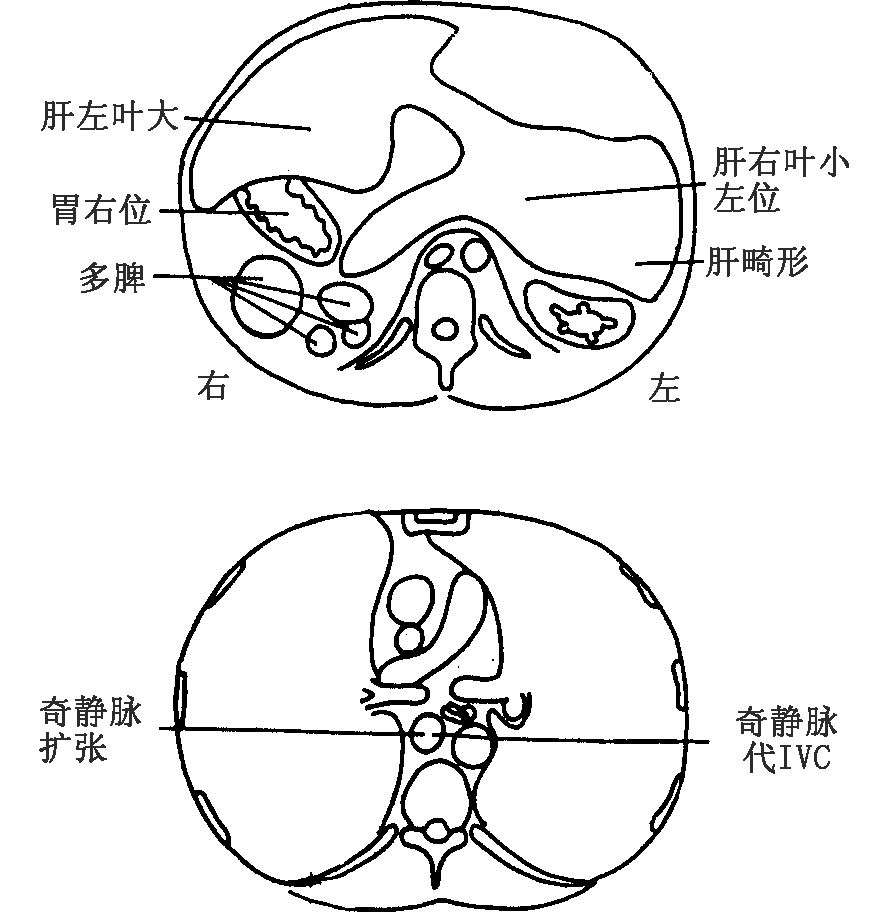
\includegraphics[width=.7\textwidth,height=\textheight,keepaspectratio]{./images/Image00311.jpg}
 \captionsetup{justification=centering}
 \caption{多脾合并多种畸形}
 \label{fig14-3}
  \end{figure} 

\section{脾脏感染及梗死}

\subsection{脾脓肿}

本病较少见,通常是全身感染的一部分。

\textbf{【病因病理】}
一般为细菌感染,免疫力低下者则可为真菌感染。75%经血行播散、15%由于脾损伤、10%由于脾梗死所致。很少由邻近器官感染直接侵犯所致。早期以急性炎症反应为主,表现为脾弥漫性增大;随后炎症反应趋于局限化,进而形成脓肿。脓肿可单房或多房、多发或单发、大小不等。

\textbf{【临床表现】}
常存在败血症症状,出现发热、寒颤、左上腹痛、脾大、恶心、呕吐、白细胞增高等。但临床确诊困难,极易漏诊。

\textbf{【CT表现】}
脓肿呈圆形或椭圆形低密度区,CT值为20Hu左右,多<30Hu,境界不清;脓腔内有气-液面或液-液面是其可靠表现。增强扫描脓肿壁强化明显,内壁光整,壁外有水肿带;当脓肿为多发而又较小时,则常表现为增强的脾内有斑点状或粟粒状充盈缺损现象。可并发脾周及膈下积液,甚至脾破裂;还可见左侧肾前筋膜增厚。

\subsection{脾结核}

本病罕见,通常继发于肺结核。感染途径以血行为主。

\textbf{【病理】}
①粟粒型脾结核:最初产生渗出性病变,病灶广泛即形成“粟粒型脾结核”。②结节型脾结核:渗出病灶如不吸收,可发展成结核性肉芽肿,并发生干酪坏死,直径多在5~20mm大小,形成“结节型脾结核”,即所谓的大结节。③结核性脾脓肿:当结节性病灶相互融合或孤立性病灶发展增大,并液化形成“结核性脾脓肿”。④脾结核钙化:钙化灶大多在干酪性病灶的愈合过程中产生。

\textbf{【临床表现】}
多见于中青年。多有肺结核,患者全身情况差,消瘦、乏力、发热、脾大、腹痛、脾区明显压痛,常合并其他脏器结核。临床确诊困难。

\textbf{【CT表现】} 根据病理基础其CT表现亦可归纳为以下几型:

1.粟粒型脾结核:由于病灶多<2mm,CT难以显示或仅表现为脾脏的轻中度增大,密度稍低或不均。

2.结节型脾结核:该型CT显示率较高,表现为边界不清、大小不等的多发低或等密度灶;增强后多无强化,边界清楚,少数可见环状强化(肉芽组织)。

3.结核性脾脓肿:表现为脾内单发或多发较大类圆形低密度灶;增强后边缘强化而内部无强化。

4.脾结核钙化:多表现为1~5mm的斑点状高密度灶(图\ref{fig14-4})。结节型脾结核愈合钙化可表现为花冠状或羊毛状钙化。

\begin{figure}[!htbp]
 \centering
 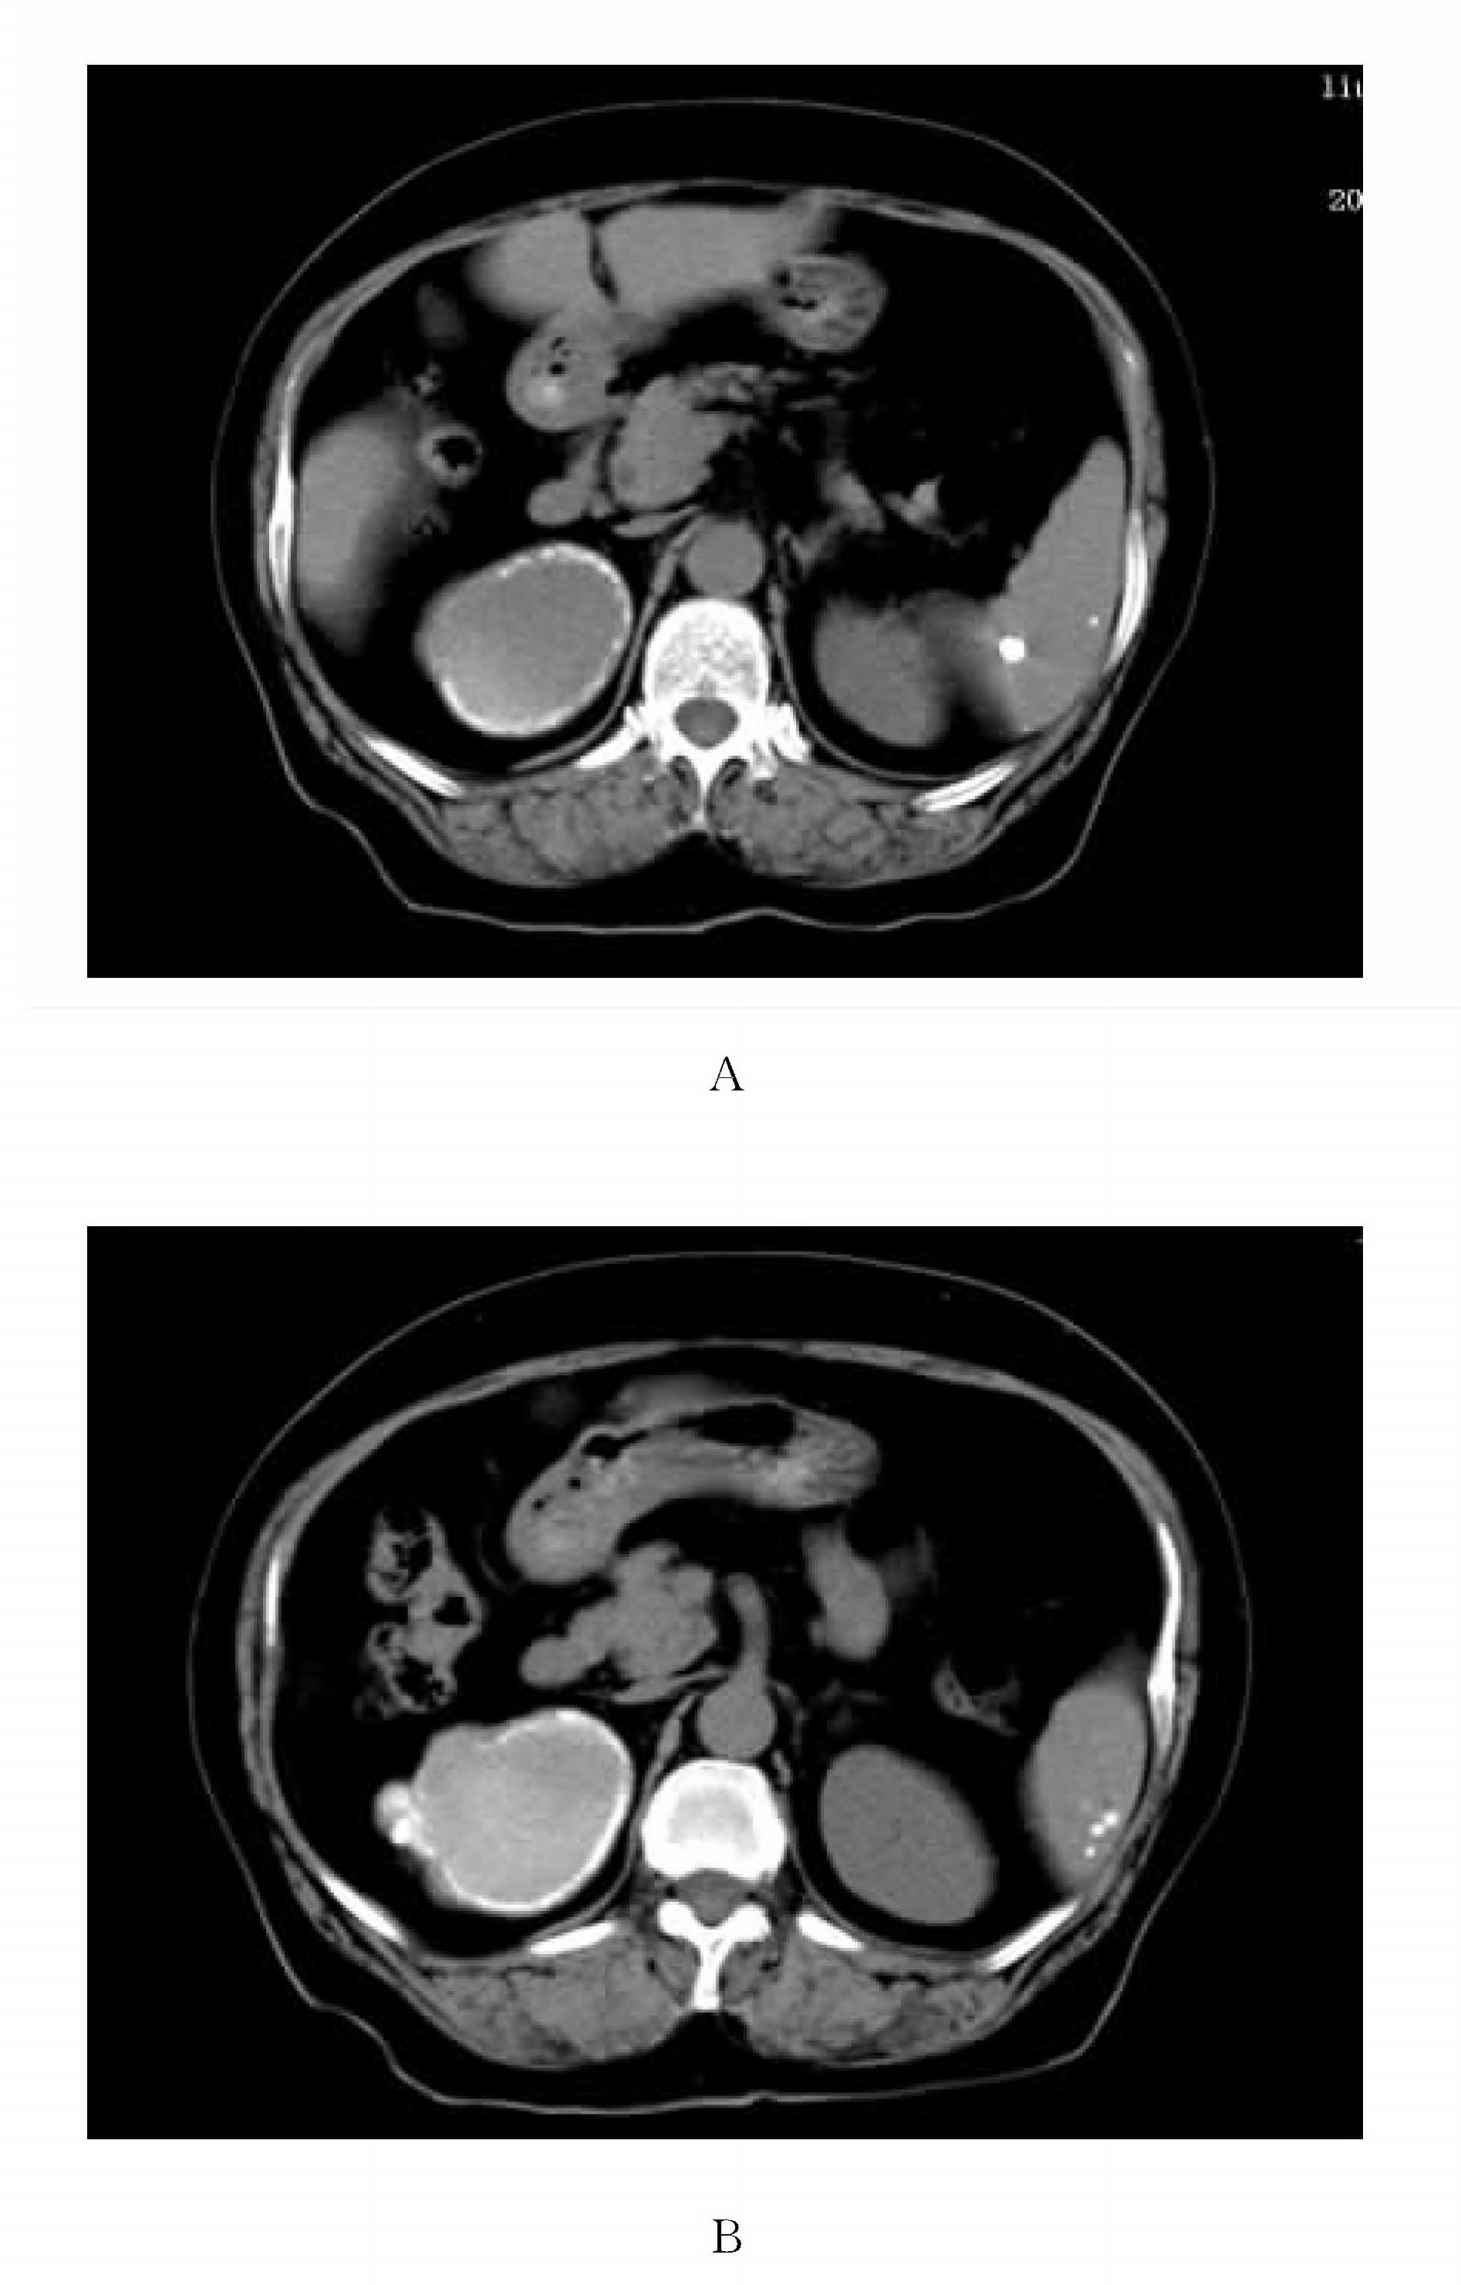
\includegraphics[width=.7\textwidth,height=\textheight,keepaspectratio]{./images/Image00312.jpg}
 \captionsetup{justification=centering}
 \caption{脾结核(钙化)\\{\small A、B为同一患者,脾脏内有多个沙粒状钙化,合并右肾结核}}
 \label{fig14-4}
  \end{figure} 

此外,还可见腹膜后、肝门、脾门淋巴结增大、钙化、环状强化,以及其他器官(如肺、肝、胰、肾上腺、肠和脊椎等)结核。

\textbf{【诊断要点】}
①好发于20~25岁,多数伴结核中毒症状;②CT平扫见脾内弥漫性低密度灶,直径多<20mm;增强后病灶无强化;③多伴有腹膜后和肝门等淋巴结增大、钙化或周边环状强化;④常伴其他脏器结核;⑤脾内散在斑点样钙化,直径1~5mm大小。

\textbf{【鉴别诊断】}

1.淋巴瘤:是脾最常见的原发性肿瘤,临床与脾结核无明显区别。但淋巴瘤常为多发或单发,弥漫性病变较少,无钙化和其他脏器结核;增强后病灶轻度强化,增大淋巴结多无环状强化。再结合临床、骨髓象、血象等做出诊断。

2.转移瘤:多有原发肿瘤史。CT表现为脾内单发或多发的低密度灶,少有弥漫性;病灶相对较大,可出现“牛眼征”或“靶心征”;淋巴结多无环状强化等有助于诊断。

3.脾脓肿:临床表现为寒颤、高热及白细胞计数升高。CT表现为单发或多发较大低密度灶;脓肿壁强化明显,内壁光整,壁外有水肿带等多可鉴别。

但孤立性球形脾结核仍较难与脾脏恶性肿瘤相鉴别,应予重视。

\subsection{脾结节病}

本病多为全身结节病的局部病变,但偶可孤立发生于脾脏。

\textbf{【CT表现】}
脾内病灶呈低密度团块状病灶,可多发、亦可单发。CT值约30~40Hu;增强扫描呈轻度强化,与显著强化的脾界限更清晰。为全身结节病的一部分时,可见胸部结节病的相应表现。

\subsection{脾梗死}

本病是指脾内动脉的分支阻塞,造成局部脾组织的缺血坏死。

\textbf{【病因病理】}
其病因主要有血栓形成、动脉粥样硬化、二尖瓣疾病、溶血性贫血、白血病、结缔组织疾病、脾动脉瘤等。当门静脉高压脾大时,更易发生梗死。其病理学变化为贫血性梗死,但在脾淤血时,病灶周围有出血带。晚期坏死脾组织被纤维组织所代替,因纤维瘢痕收缩,使脾脏局部凹陷。较大的梗死灶,不能完全纤维化,其中央可发生液化,并被纤维结缔组织包裹形成囊腔。

\textbf{【临床表现】}
多无症状,有时可出现左上腹痛、左膈升高、左侧胸腔积液。

\textbf{【CT表现】}
梗死多发生于脾前缘处近脾门方向,大小不等,常多个病灶同时存在。梗死灶呈三角形或楔形,底在脾的外缘,尖端指向脾门(图\ref{fig14-5})。有时呈不规则形低密度灶。但病程少于5天者多呈等密度而不易显示。增强扫描因不强化而显示更清楚。若整个脾脏梗死,则只有包膜强化表现。在急性期(8天以前)呈低密度区、不强化;慢性期(15~28天)则密度逐渐恢复正常,由于瘢痕收缩而出现收缩变形,甚至合并钙化。不典型者呈多发的、不均匀的、边缘不清楚的小片状或大片状低密度区。大的梗死灶中央可以伴有囊性变。少数伴有包膜下积液。

\begin{figure}[!htbp]
 \centering
 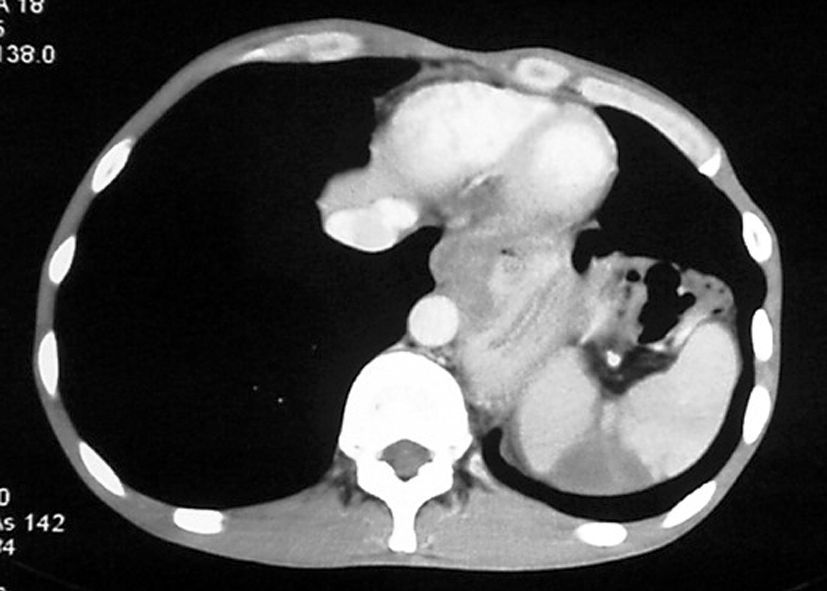
\includegraphics[width=.7\textwidth,height=\textheight,keepaspectratio]{./images/Image00313.jpg}
 \captionsetup{justification=centering}
 \caption{脾梗死\\{\small 食管癌术后复发且并发脾梗死,增强扫描脾内有楔形低密度区,尖端指向肺门}}
 \label{fig14-5}
  \end{figure} 

\subsection{弥漫性脾大}

脾脏的大小、形态差异较大,无论是临床查体还是CT确定其大小有时较为困难。儿童脾脏的大小可用公式计算,即L(cm)=5.7+0.31A(L是脾脏的长轴,A为年龄)。到达青春期脾脏的大小和重量可以达到最大。

\textbf{【病因】} 弥漫性脾大的病因主要有以下几方面:

1.感染性疾病:可引起脾脏非特异性增大,如败血症、亚急性细菌性心内膜炎、肠伤寒、传染性单核细胞增多症、巨细胞病毒感染以及寄生虫病(如疟疾、血吸虫病)、肉芽肿性病变(如结核、组织胞浆菌病、结节病)等。它们在急性期可引起脾大,慢性期可正常大小。

2.血液系统疾病:可引起脾大,特别是骨髓增生性病变、霍奇金病弥漫性浸润、真性红细胞增多症、骨髓纤维化、骨髓外化生等。其他如淋巴细胞性白血病、自身免疫性贫血、血小板减少性紫癜、遗传性球形红细胞增多症。异形镰状细胞病患者脾亦可增大,但常伴反复梗死和血肿,反复梗死最终导致自截(萎缩)。

3.充血性脾增大:见于门静脉高压或脾静脉的阻塞和血栓形成,以及心脏病。

4.结缔组织疾病:如系统性红斑狼疮、风湿性关节炎等。

此外,代谢性疾病如类脂质沉积症(高雪氏病、尼曼-匹克病)、糖尿病等也可导致脾大。淀粉样变亦可出现脾大(但CT脾内可见多发性低密度结节、弥漫性密度减低,强化亦很轻微)。

\textbf{【CT表现】}
脾脏的长>15cm肯定增大,脾厚>4.5cm可视为增大。此外,脾脏的下缘超过正常肝脏的下缘或脾脏前后径超过腹部前后径的2/3均提示脾大。我们认为利用肋单元判断脾脏大小(正常为5个以下肋单元)存在严重不足,准确性甚差。脾脏的容积测量虽然更加接近实际大小,但因个体差异较大,以及影响因素较多,仍难分辨正常与轻度异常。

\subsection{脾内钙化的鉴别诊断}

识别脾内钙化有助于脾脏疾病的鉴别诊断。引起脾内钙化的疾病较多:①肉芽肿(如结核、组织胞浆菌病)是最常见的,呈点状,可伴肝或肺内钙化。②脾附近或脾内静脉石见于血管性异常,如血管瘤病。③脾周边的环形钙化见于陈旧性血肿或动脉瘤。脾动脉、脾动脉瘤的钙化可呈曲线状,常见于脾门部,钙化的动脉瘤较未钙化者不易破裂。④脾包虫囊肿仅在明确囊内容物(如子囊)时方可诊断。⑤卡氏肺囊虫感染引起的脾钙化亦有报道。⑥脾梗死的钙化可发生在镰状细胞性贫血的病人,但不常见。此外,除脾外,肾及淋巴结亦可见钙化。

\section{脾囊肿及肿瘤}

\subsection{概述}

1.良性肿瘤:很少见,有血管瘤、淋巴管瘤、血管淋巴管瘤(亦称为脉管瘤)和错构瘤。更少见的有纤维瘤、平滑肌瘤、神经纤维瘤、脂肪瘤等。

2.恶性肿瘤:脾原发性恶性肿瘤极少见,以恶性淋巴瘤和血管内皮肉瘤较常见。罕见的有梭形细胞肉瘤、平滑肌肉瘤、纤维肉瘤、恶性神经纤维肉瘤、卡波西氏肉瘤(Kaposi肉瘤)、淋巴管内皮肉瘤、恶性组织细胞增生症等。

\subsection{脾囊肿}

\textbf{【病因病理】}
①真性囊肿:内衬以内皮细胞,系先天性囊肿。②假性囊肿:即继发性囊肿,多见,占脾囊肿的80%。囊壁无内皮细胞被覆,大多为外伤后血肿退变所致,也可见于脾梗死后及胰腺炎所致。③包虫性囊肿:占全部包囊虫病的2%~3%,多与肝、肺等脏器的病变同时发生。

\textbf{【临床表现】}
多见于40岁以下,男女发病率之比约为2∶1。小的囊肿多无症状。只有当囊肿巨大压迫胃、左肾和输尿管等邻近脏器时,产生相应的压迫症状或局部触及肿块。

\textbf{【CT表现】}
平扫呈圆形或椭圆形的水样低密度灶,界限清楚,有时可多发(图\ref{fig14-6})。先天性囊肿壁很薄,外形规则;假性囊肿壁可稍厚及稍不规则。囊壁有时钙化,先天性囊壁钙化细而光滑;后天性则厚而欠规则;胰腺炎所致者常在囊肿边缘见到裂隙,有一定特征。包虫囊肿往往使脾增大,囊液CT值较前两者稍高,囊内可有钙化;也可见到囊内子囊、双边征及水上荷花征和飘带征等。增强扫描先天性及假性囊肿囊壁不强化。包虫囊肿也不强化,但当有脱落的内囊及子囊存在时,则有囊壁强化表现。

\begin{figure}[!htbp]
 \centering
 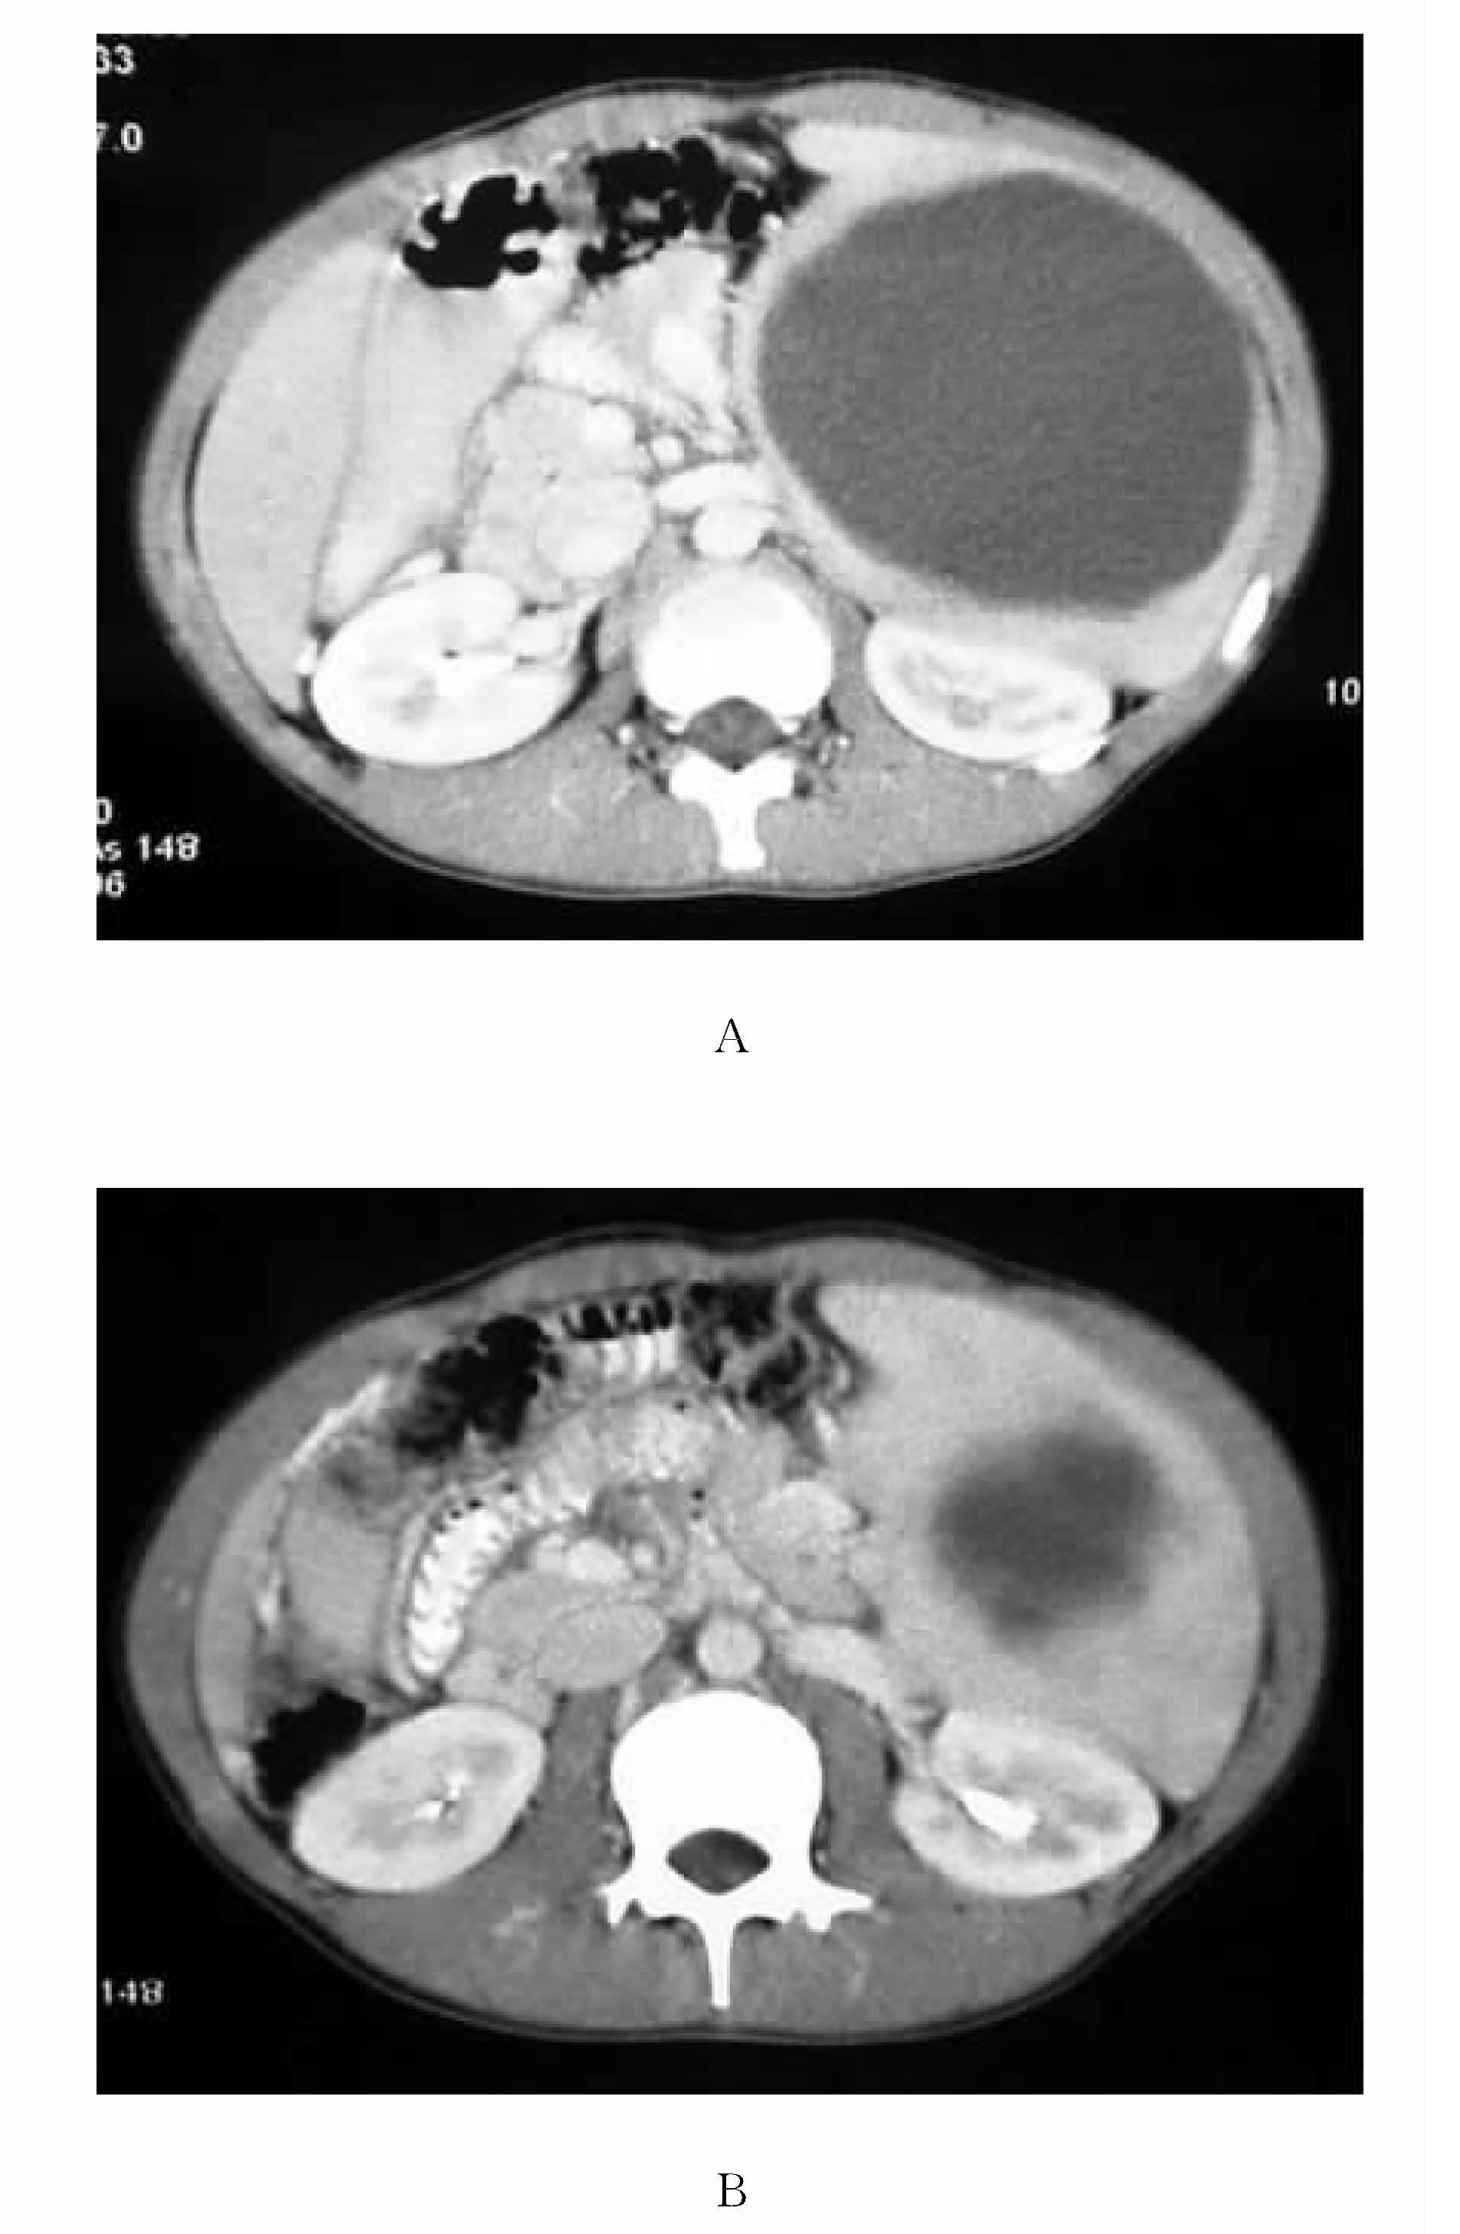
\includegraphics[width=.7\textwidth,height=\textheight,keepaspectratio]{./images/Image00314.jpg}
 \captionsetup{justification=centering}
 \caption{脾囊肿\\{\small A、B为同一患者,脾内有巨大圆形水样密度灶,边缘光滑,无强化}}
 \label{fig14-6}
  \end{figure} 

\subsection{脾血管瘤}

本病是最常见的脾良性肿瘤。

\textbf{【病理】}
与其他部位的血管瘤类似,多为海绵样或毛细血管样扩张的血管构成。单发或多发,瘤内可有栓塞、出血、纤维化或钙化。肿瘤生长缓慢。

\textbf{【临床表现】}
多见于20~50岁,男性多于女性,偶见于儿童。通常无症状。大的血管瘤可有左上腹包块、胀痛及邻近脏器受压症状;亦可发生破裂而出现急性腹痛、血压下降和休克等;偶有脾亢症状。

\textbf{【CT表现】}
肿瘤直径多<2cm,>5cm者少见,较大的血管瘤可致脾增大。平扫呈低密度或等密度肿块,可有少许钙化存在或中心见更低密度瘢痕区。偶呈囊样,但壁厚。增强扫描病灶均匀强化,亦偶可不均匀强化。快速增强扫描亦可见边缘明显结节状强化,然后逐渐向中心充填,延迟扫描大多完全填充而呈等密度。总之,其表现与肝血管瘤相类似是其特征。

\subsection{脾淋巴管瘤}

脾脏淋巴管瘤是非常少见的先天性畸形。

\textbf{【病理】}
淋巴管瘤组织学上根据异常淋巴管扩张后的大小不同分为毛细管型、海绵状型和囊肿型3类,以囊肿型最常见。多位于颈、腋窝、纵隔、腹膜后和四肢软组织内。脾脏罕见,可单发、多发或弥漫分布于整个脾脏。

\textbf{【临床表现】}
脾脏淋巴管瘤多见于中青年。感觉左上腹部胀满或轻微胀痛,个别无症状。脾脏可增大。

\textbf{【CT表现】}
脾脏增大。脾内有单发或多发大小不等的近水样低密度灶,CT值约10~30Hu。囊内可见小片状稍高密度灶(可能与含铁血黄素有关)。有文献认为如囊内为脂肪液体则是淋巴管瘤的特征性改变。病灶边缘清楚,周边及间隔增强后有轻度强化,与脾囊肿不同。可合并感染、出血和钙化。

\textbf{【鉴别诊断】}
病灶CT值偏高,内有粗间隔和边缘轻度强化可与囊肿鉴别。脓肿壁强化显著、外周有水肿,两者亦不难鉴别。

\subsection{脾脉管瘤}

脉管瘤是血管瘤和淋巴管瘤的混合瘤,脾脉管瘤较为罕见。国内有学者报道1例脾弥漫性脉管瘤,甚为少见。

\textbf{【CT表现】}
①脾大,表面可凹凸不平,包膜完整。②脾内可见多个大小不等的类圆形低密度结节,直径0.5~3.0cm。因血管和淋巴管成分的多少而密度不一,但多>30Hu。大多界限不清(表明血管成分多),少部分边缘清晰锐利(表明血管成分少)。③增强扫描因血管成分的多少而呈中度强化,部分强化不著。④多发时整个脾脏呈蜂窝状,病灶为蜂巢、脾实质为瘤巢的支架。

\textbf{【鉴别诊断】}
根据上述特点且多无增大淋巴结等可与多发且具有“牛眼征”或“靶征”的转移瘤相鉴别。根据其密度、边缘与强化表现也可与囊性淋巴管瘤相鉴别。

\subsection{脾错构瘤}

本病较为罕见,是由于异常数量和杂乱排列的正常组织(如脾、血管、脂肪和平滑肌等组织)构成的肿瘤样畸形。

\textbf{【病理】}
可能来源于脾始基局限性发育障碍,使正常成分的脾组织(如脾、血管、脂肪组织、纤维组织和平滑肌等)组合比例发生混乱。多为单发,偶可多发。无包膜,大小为数毫米到15mm以上。

\textbf{【临床表现】}
成人多见,少数见于儿童;女性略多见。多无症状,少数大者有左上腹不适,疼痛,偶有脾亢。

\textbf{【CT表现】}
多为单发低密度实性病灶,偶为囊实性或囊性病灶,轮廓多不清。偶见星状或团块状粗糙钙化,如含脂肪组织,CT值<-25Hu较有特征。增强扫描多呈弥漫性渐进性较明显强化,并呈延迟强化现象。总之,伴有钙化和脂肪组织的肿块为其特征性表现。

\subsection{脾血管内皮肉瘤}

本病又称为脾血管内皮瘤,是起源于脾窦内皮细胞的高度恶性肿瘤,很少见。

\textbf{【临床表现】}
左上腹疼痛、发热,很快出现左上腹肿块;恶病质状态明显;常早期转移到肝、肺、骨骼、腹膜等处。有时可发生脾自发性破裂。此病预后差。

\textbf{【CT表现】}
①脾脏增大。②脾内单发或多发大小不等、边界较清的实性或囊实性结节状低密度灶,有时可见出血征象。当肿块内含有钙化或含铁血黄素沉着时,CT值可高达100Hu以上。③常见腹水。④增强扫描可见脾内多发的成簇状强化区存在,并有向病灶中心扩展的趋势。常占据脾的大部分,坏死囊变区不强化。⑤可有其他脏器及腹膜后淋巴结转移表现。⑥若有自发破裂可出现包膜下或脾周出血表现。

\subsection{脾淋巴瘤}

本病绝大多数为全身淋巴瘤对脾脏的浸润,原发性极少。NHL约67%的病例脾脏受累,HD约70%有脾浸润。原发性75%为NHL。

\textbf{【病理】}
脾淋巴瘤大体病理分为4种类型:①均匀弥漫型:脾均匀弥漫性增大,无明显肿块形成;②粟粒结节型:病灶为1~5mm大小;③多发肿块型:病灶2~10cm大小;④巨块型:病灶大于10cm。

\textbf{【临床表现】}
多表现为发热、贫血、乏力、纳差、体重下降、左上腹痛,脾脏增大、边缘有结节感。全身淋巴瘤可有全身广泛淋巴结肿大。白细胞和血小板可减少。

\textbf{【CT表现】}
综合有关文献其CT表现分为4类:①弥漫增大型:表现为脾脏显著增大,密度较均匀。如NHL脾明显增大,高度提示淋巴瘤侵犯。但脾大并不一定意味着有脾内淋巴瘤,脾不大却可能有淋巴瘤侵犯。②弥漫细小结节型:脾大小也可正常。脾内弥漫性低密度小结节,大小为0.2~1.0cm。但<1.0cm的结节平扫甚至增强扫描亦难以显示,而仅表现为脾大。③结节型:呈圆形或类圆形、单发或多发低密度结节,结节直径>1.0cm。④块状型:单发或多发的、直径>3.0cm的低密度肿块。

总之,脾淋巴瘤CT表现为脾大、脾内弥漫多发或单发(但单发少见)低密度肿块或结节,边界不清,无钙化及出血。增强扫描脾明显强化,而肿块或结节多强化不明显。继发性常伴脾门及腹膜后淋巴结增大。

\textbf{【鉴别诊断】}

1.血管内皮肉瘤:表现为脾大,常伴腹水。平扫示脾内大小不等、单发或多发实性或囊实性混合密度肿块,肿块内常有出血或钙化,边界清晰。增强扫描见脾内成簇状多发的强化区存在。此外,肿瘤破裂可引起脾包膜下及腹腔积血。

2.脾梗死:多发生于脾前缘近脾门方向,病灶常呈楔形,尖端指向脾门,无强化,可伴脾内出血。

3.转移瘤:常有明确的原发灶,多发生于全身广泛转移的晚期。CT表现为脾大,脾内单发或多发的低密度灶,境界清晰。伴有肝和其他脏器的转移和腹水。

此外,应注意结合临床与引起脾大的其他疾病如白血病等相鉴别。

\subsection{脾转移瘤}

脾转移瘤远较肝脏少见,其原因主要是脾为具有免疫监督能力的特殊器官,但也有文献认为可能与肝有门静脉系统有关。有人认为脾脏转移时,一般都有多个器官受累。常见的原发肿瘤依次为肺癌、乳癌、前列腺癌、结肠癌、恶性黑色素瘤、卵巢癌、宫颈癌和胰腺癌。多为血行转移,少数为直接侵犯和种植。

\textbf{【病理】}
病灶可位于脾脏的静脉窦、红髓、白髓和小梁血管等处。病灶大小不等,呈结节型或弥漫型。大的结节可伴有坏死液化。广泛转移可伴脾弥漫性增大。

\textbf{【临床表现】}
大多有肿瘤病史。常伴有消瘦、乏力、低热、贫血等恶性肿瘤的晚期表现,少数可有左上腹疼痛不适。体检脾脏增大。

\textbf{【CT表现】}
呈多样化,缺乏特异性。脾脏轻度增大或不大。脾内单发或多发、大小不等的低密度灶,边缘清楚或不清楚(图\ref{fig14-7});也可呈囊性或囊实性,少数呈等密度。微小结节和弥漫性脾浸润CT不能发现。邻近器官病变的直接浸润表现为肿块与脾的界限消失或脾边缘密度减低。增强扫描有轻度不均匀强化,病灶密度低于脾实质。多同时可见肝脏或其他脏器转移灶。

\begin{figure}[!htbp]
 \centering
 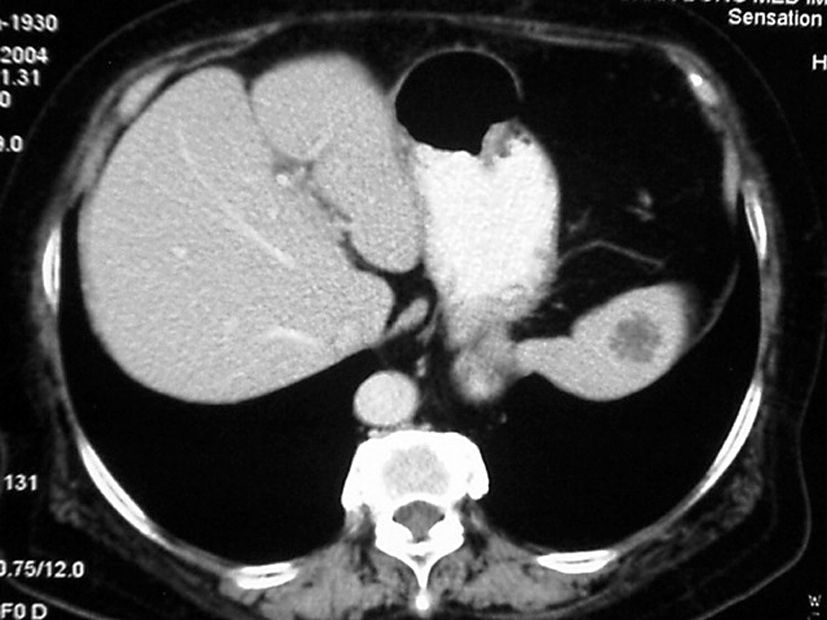
\includegraphics[width=.7\textwidth,height=\textheight,keepaspectratio]{./images/Image00315.jpg}
 \captionsetup{justification=centering}
 \caption{脾转移瘤\\{\small 为结肠癌脾转移。增强扫描平衡期,脾脏内有一欠规则低密度灶,边缘呈不规则强化}}
 \label{fig14-7}
  \end{figure} 

\textbf{【鉴别诊断】}
脾囊性转移尤其是单发者应与囊肿相鉴别。前者囊壁多较厚,且有强化和壁结节,结合肝内等转移灶可予鉴别。还应注意结合病史与淋巴瘤相鉴别。

\protect\hypertarget{text00022.html}{}{}

